% Options for packages loaded elsewhere
% Options for packages loaded elsewhere
\PassOptionsToPackage{unicode}{hyperref}
\PassOptionsToPackage{hyphens}{url}
\PassOptionsToPackage{dvipsnames,svgnames,x11names}{xcolor}
%
\documentclass[
  letterpaper,
]{tufte-book}
\usepackage{xcolor}
\usepackage{amsmath,amssymb}
\setcounter{secnumdepth}{5}
\usepackage{iftex}
\ifPDFTeX
  \usepackage[T1]{fontenc}
  \usepackage[utf8]{inputenc}
  \usepackage{textcomp} % provide euro and other symbols
\else % if luatex or xetex
  \usepackage{unicode-math} % this also loads fontspec
  \defaultfontfeatures{Scale=MatchLowercase}
  \defaultfontfeatures[\rmfamily]{Ligatures=TeX,Scale=1}
\fi
\usepackage[]{palatino}
\ifPDFTeX\else
  % xetex/luatex font selection
  \setmainfont[]{ETbb}
  \setsansfont[Scale=MatchUppercase]{TeX Gyre Heros}
\fi
% Use upquote if available, for straight quotes in verbatim environments
\IfFileExists{upquote.sty}{\usepackage{upquote}}{}
\IfFileExists{microtype.sty}{% use microtype if available
  \usepackage[]{microtype}
  \UseMicrotypeSet[protrusion]{basicmath} % disable protrusion for tt fonts
}{}
\makeatletter
\@ifundefined{KOMAClassName}{% if non-KOMA class
  \IfFileExists{parskip.sty}{%
    \usepackage{parskip}
  }{% else
    \setlength{\parindent}{0pt}
    \setlength{\parskip}{6pt plus 2pt minus 1pt}}
}{% if KOMA class
  \KOMAoptions{parskip=half}}
\makeatother
% Make \paragraph and \subparagraph free-standing
\makeatletter
\ifx\paragraph\undefined\else
  \let\oldparagraph\paragraph
  \renewcommand{\paragraph}{
    \@ifstar
      \xxxParagraphStar
      \xxxParagraphNoStar
  }
  \newcommand{\xxxParagraphStar}[1]{\oldparagraph*{#1}\mbox{}}
  \newcommand{\xxxParagraphNoStar}[1]{\oldparagraph{#1}\mbox{}}
\fi
\ifx\subparagraph\undefined\else
  \let\oldsubparagraph\subparagraph
  \renewcommand{\subparagraph}{
    \@ifstar
      \xxxSubParagraphStar
      \xxxSubParagraphNoStar
  }
  \newcommand{\xxxSubParagraphStar}[1]{\oldsubparagraph*{#1}\mbox{}}
  \newcommand{\xxxSubParagraphNoStar}[1]{\oldsubparagraph{#1}\mbox{}}
\fi
\makeatother

\usepackage{color}
\usepackage{fancyvrb}
\newcommand{\VerbBar}{|}
\newcommand{\VERB}{\Verb[commandchars=\\\{\}]}
\DefineVerbatimEnvironment{Highlighting}{Verbatim}{commandchars=\\\{\}}
% Add ',fontsize=\small' for more characters per line
\usepackage{framed}
\definecolor{shadecolor}{RGB}{241,243,245}
\newenvironment{Shaded}{\begin{snugshade}}{\end{snugshade}}
\newcommand{\AlertTok}[1]{\textcolor[rgb]{0.68,0.00,0.00}{#1}}
\newcommand{\AnnotationTok}[1]{\textcolor[rgb]{0.37,0.37,0.37}{#1}}
\newcommand{\AttributeTok}[1]{\textcolor[rgb]{0.40,0.45,0.13}{#1}}
\newcommand{\BaseNTok}[1]{\textcolor[rgb]{0.68,0.00,0.00}{#1}}
\newcommand{\BuiltInTok}[1]{\textcolor[rgb]{0.00,0.23,0.31}{#1}}
\newcommand{\CharTok}[1]{\textcolor[rgb]{0.13,0.47,0.30}{#1}}
\newcommand{\CommentTok}[1]{\textcolor[rgb]{0.37,0.37,0.37}{#1}}
\newcommand{\CommentVarTok}[1]{\textcolor[rgb]{0.37,0.37,0.37}{\textit{#1}}}
\newcommand{\ConstantTok}[1]{\textcolor[rgb]{0.56,0.35,0.01}{#1}}
\newcommand{\ControlFlowTok}[1]{\textcolor[rgb]{0.00,0.23,0.31}{\textbf{#1}}}
\newcommand{\DataTypeTok}[1]{\textcolor[rgb]{0.68,0.00,0.00}{#1}}
\newcommand{\DecValTok}[1]{\textcolor[rgb]{0.68,0.00,0.00}{#1}}
\newcommand{\DocumentationTok}[1]{\textcolor[rgb]{0.37,0.37,0.37}{\textit{#1}}}
\newcommand{\ErrorTok}[1]{\textcolor[rgb]{0.68,0.00,0.00}{#1}}
\newcommand{\ExtensionTok}[1]{\textcolor[rgb]{0.00,0.23,0.31}{#1}}
\newcommand{\FloatTok}[1]{\textcolor[rgb]{0.68,0.00,0.00}{#1}}
\newcommand{\FunctionTok}[1]{\textcolor[rgb]{0.28,0.35,0.67}{#1}}
\newcommand{\ImportTok}[1]{\textcolor[rgb]{0.00,0.46,0.62}{#1}}
\newcommand{\InformationTok}[1]{\textcolor[rgb]{0.37,0.37,0.37}{#1}}
\newcommand{\KeywordTok}[1]{\textcolor[rgb]{0.00,0.23,0.31}{\textbf{#1}}}
\newcommand{\NormalTok}[1]{\textcolor[rgb]{0.00,0.23,0.31}{#1}}
\newcommand{\OperatorTok}[1]{\textcolor[rgb]{0.37,0.37,0.37}{#1}}
\newcommand{\OtherTok}[1]{\textcolor[rgb]{0.00,0.23,0.31}{#1}}
\newcommand{\PreprocessorTok}[1]{\textcolor[rgb]{0.68,0.00,0.00}{#1}}
\newcommand{\RegionMarkerTok}[1]{\textcolor[rgb]{0.00,0.23,0.31}{#1}}
\newcommand{\SpecialCharTok}[1]{\textcolor[rgb]{0.37,0.37,0.37}{#1}}
\newcommand{\SpecialStringTok}[1]{\textcolor[rgb]{0.13,0.47,0.30}{#1}}
\newcommand{\StringTok}[1]{\textcolor[rgb]{0.13,0.47,0.30}{#1}}
\newcommand{\VariableTok}[1]{\textcolor[rgb]{0.07,0.07,0.07}{#1}}
\newcommand{\VerbatimStringTok}[1]{\textcolor[rgb]{0.13,0.47,0.30}{#1}}
\newcommand{\WarningTok}[1]{\textcolor[rgb]{0.37,0.37,0.37}{\textit{#1}}}

\usepackage{longtable,booktabs,array}
\usepackage{calc} % for calculating minipage widths
% Correct order of tables after \paragraph or \subparagraph
\usepackage{etoolbox}
\makeatletter
\patchcmd\longtable{\par}{\if@noskipsec\mbox{}\fi\par}{}{}
\makeatother
% Allow footnotes in longtable head/foot
\IfFileExists{footnotehyper.sty}{\usepackage{footnotehyper}}{\usepackage{footnote}}
\makesavenoteenv{longtable}
\usepackage{graphicx}
\makeatletter
\newsavebox\pandoc@box
\newcommand*\pandocbounded[1]{% scales image to fit in text height/width
  \sbox\pandoc@box{#1}%
  \Gscale@div\@tempa{\textheight}{\dimexpr\ht\pandoc@box+\dp\pandoc@box\relax}%
  \Gscale@div\@tempb{\linewidth}{\wd\pandoc@box}%
  \ifdim\@tempb\p@<\@tempa\p@\let\@tempa\@tempb\fi% select the smaller of both
  \ifdim\@tempa\p@<\p@\scalebox{\@tempa}{\usebox\pandoc@box}%
  \else\usebox{\pandoc@box}%
  \fi%
}
% Set default figure placement to htbp
\def\fps@figure{htbp}
\makeatother


% definitions for citeproc citations
\NewDocumentCommand\citeproctext{}{}
\NewDocumentCommand\citeproc{mm}{%
  \begingroup\def\citeproctext{#2}\cite{#1}\endgroup}
\makeatletter
 % allow citations to break across lines
 \let\@cite@ofmt\@firstofone
 % avoid brackets around text for \cite:
 \def\@biblabel#1{}
 \def\@cite#1#2{{#1\if@tempswa , #2\fi}}
\makeatother
\newlength{\cslhangindent}
\setlength{\cslhangindent}{1.5em}
\newlength{\csllabelwidth}
\setlength{\csllabelwidth}{3em}
\newenvironment{CSLReferences}[2] % #1 hanging-indent, #2 entry-spacing
 {\begin{list}{}{%
  \setlength{\itemindent}{0pt}
  \setlength{\leftmargin}{0pt}
  \setlength{\parsep}{0pt}
  % turn on hanging indent if param 1 is 1
  \ifodd #1
   \setlength{\leftmargin}{\cslhangindent}
   \setlength{\itemindent}{-1\cslhangindent}
  \fi
  % set entry spacing
  \setlength{\itemsep}{#2\baselineskip}}}
 {\end{list}}
\usepackage{calc}
\newcommand{\CSLBlock}[1]{\hfill\break\parbox[t]{\linewidth}{\strut\ignorespaces#1\strut}}
\newcommand{\CSLLeftMargin}[1]{\parbox[t]{\csllabelwidth}{\strut#1\strut}}
\newcommand{\CSLRightInline}[1]{\parbox[t]{\linewidth - \csllabelwidth}{\strut#1\strut}}
\newcommand{\CSLIndent}[1]{\hspace{\cslhangindent}#1}



\setlength{\emergencystretch}{3em} % prevent overfull lines

\providecommand{\tightlist}{%
  \setlength{\itemsep}{0pt}\setlength{\parskip}{0pt}}



 


\makeatletter
\@ifpackageloaded{bookmark}{}{\usepackage{bookmark}}
\makeatother
\makeatletter
\@ifpackageloaded{caption}{}{\usepackage{caption}}
\AtBeginDocument{%
\ifdefined\contentsname
  \renewcommand*\contentsname{Table of contents}
\else
  \newcommand\contentsname{Table of contents}
\fi
\ifdefined\listfigurename
  \renewcommand*\listfigurename{List of Figures}
\else
  \newcommand\listfigurename{List of Figures}
\fi
\ifdefined\listtablename
  \renewcommand*\listtablename{List of Tables}
\else
  \newcommand\listtablename{List of Tables}
\fi
\ifdefined\figurename
  \renewcommand*\figurename{Figure}
\else
  \newcommand\figurename{Figure}
\fi
\ifdefined\tablename
  \renewcommand*\tablename{Table}
\else
  \newcommand\tablename{Table}
\fi
}
\@ifpackageloaded{float}{}{\usepackage{float}}
\floatstyle{ruled}
\@ifundefined{c@chapter}{\newfloat{codelisting}{h}{lop}}{\newfloat{codelisting}{h}{lop}[chapter]}
\floatname{codelisting}{Listing}
\newcommand*\listoflistings{\listof{codelisting}{List of Listings}}
\usepackage{amsthm}
\theoremstyle{definition}
\newtheorem{definition}{Definition}[chapter]
\theoremstyle{remark}
\AtBeginDocument{\renewcommand*{\proofname}{Proof}}
\newtheorem*{remark}{Remark}
\newtheorem*{solution}{Solution}
\newtheorem{refremark}{Remark}[chapter]
\newtheorem{refsolution}{Solution}[chapter]
\makeatother
\makeatletter
\makeatother
\makeatletter
\@ifpackageloaded{caption}{}{\usepackage{caption}}
\@ifpackageloaded{subcaption}{}{\usepackage{subcaption}}
\makeatother
\makeatletter
\@ifpackageloaded{sidenotes}{}{\usepackage{sidenotes}}
\@ifpackageloaded{marginnote}{}{\usepackage{marginnote}}
\makeatother
\usepackage{bookmark}
\IfFileExists{xurl.sty}{\usepackage{xurl}}{} % add URL line breaks if available
\urlstyle{same}
\hypersetup{
  pdftitle={Optimal Scheduling for Cross-Facility Workflows},
  pdfauthor={Mark Asch},
  colorlinks=true,
  linkcolor={blue},
  filecolor={Maroon},
  citecolor={Blue},
  urlcolor={Blue},
  pdfcreator={LaTeX via pandoc}}


\title{Optimal Scheduling for Cross-Facility Workflows}
\usepackage{etoolbox}
\makeatletter
\providecommand{\subtitle}[1]{% add subtitle to \maketitle
  \apptocmd{\@title}{\par {\large #1 \par}}{}{}
}
\makeatother
\subtitle{XWF for CDT}
\author{Mark Asch}
\date{2026-01-26}
\begin{document}
\frontmatter
\maketitle

\renewcommand*\contentsname{Table of contents}
{
\hypersetup{linkcolor=}
\setcounter{tocdepth}{2}
\tableofcontents
}

\mainmatter
\bookmarksetup{startatroot}

\chapter*{Welcome}\label{welcome}
\addcontentsline{toc}{chapter}{Welcome}

\markboth{Welcome}{Welcome}

This (online) book-document contains a complete presentation of
\emph{optimal scheduling} applied to Exascale and post-Exascale
workflows. These workflows combine data acquisition, data storage, data
transfer and data analysis. The HPC components of such workflows can
incorporate a diverse range of models, including partial differential
equation solvers, algebraic solvers, AI/ML-based models, and data
analytics components, all integrated into a single process (Ferreira da
Silva et al. 2024), (Unat et al. 2025).

The objective here is to address the inherent cross-facility,
multi-domain character of these workflows. This requires a very
carefully-crafted theoretical foundation that can be readily generalized
and extended to these contexts. The material covers both the theory and
its application to practical use-cases, including real contexts with
uncertainties emanating from different causes. To understand these well,
numerous examples are provided in the form of python code snippets and
jupyter notebooks. All of these are intgerated in a \emph{digital
twin}\footnote{Known as the CDT} of the underlying cyberinfrastructure,
the so-called \emph{digital continuum}.

The Continuum Digital Twin (CDT) is defined and described in the series
of forthcoming papers (Garénaux-Gruau, Bodin, and Asch 2025a, 2025b,
2025c). For optimization and scheduling, there are numerous excellent
references. Among these we point out particularly (Birge and Louveaux
2011), (Pinedo 2022), and (Powell 2022). Most of the codes are based on
the wonderful \texttt{pyomo} framework (Bynum et al. 2021), (Hart,
Watson, and Woodruff 2011) and (Postek et al. 2025). General background
on exascale workflows can be found in (M. Asch et al. 2018).

Finally, in (Mark Asch 2022) there are basic explanations of
optimization, uncertainty quantification, inverse problems and their use
for digital twins. {\marginnote{\begin{footnotesize}This book explains
\textbf{all} the tools needed for formulating and implementing digital
twins.\end{footnotesize}}}

\section*{Author}\label{author}
\addcontentsline{toc}{section}{Author}

\markright{Author}

Mark Asch is Emeritus Professor of the Université de Picardie Jules
Verne, Mathematics department.

\url{https://markasch.github.io/DT-tbx-v1/}

\url{https://github.com/markasch/}

\url{http://masch.perso.math.cnrs.fr/}

\href{mailto:mark.asch@u-picardie.fr}{\nolinkurl{mark.asch@u-picardie.fr}}

\section*{Citation}\label{citation}
\addcontentsline{toc}{section}{Citation}

\markright{Citation}

Asch, Mark. Optimal Scheduling for Cross-Facility Workflows. Online
(2026) \url{https://markasch.github.io/RCPSP4CDT/}

\begin{Shaded}
\begin{Highlighting}[]
\NormalTok{@book\{Asch2026}
\NormalTok{    title = \{Optimal \{S\}cheduling for \{C\}ross{-}\{F\}acility \{W\}orkflows\},}
\NormalTok{    author = \{Asch, Mark\},}
\NormalTok{    url = \{https://markasch.github.io/RCPSP4CDT/\},}
\NormalTok{    year = \{2026\},}
\NormalTok{    publisher = \{Online\}}
\NormalTok{\}}
\end{Highlighting}
\end{Shaded}

\section*{License}\label{license}
\addcontentsline{toc}{section}{License}

\markright{License}

This online book is frequently updated and edited. It's content is free
to use, licensed under a
\href{https://creativecommons.org/licenses/by-nc-sa/4.0/}{Creative
Commons licence}, and the code can be found on
\href{https://github.com/markasch/RCPSP4CDT}{GitHub}. A physical copy of
the book will be available at a later date.

\textbf{License:} Creative Commons Attribution-NonCommercial-ShareAlike
4.0 International License.

\section*{References}\label{references}
\addcontentsline{toc}{section}{References}

\markright{References}

\phantomsection\label{refs}
\begin{CSLReferences}{1}{0}
\bibitem[\citeproctext]{ref-Asch2022}
Asch, Mark. 2022. \emph{A {Toolbox} for {Digital} {Twins}: {From}
{Model}-{Based} to {Data}-{Driven}}. Philadelphia, PA: Society for
Industrial; Applied Mathematics.
\url{https://doi.org/10.1137/1.9781611976977}.

\bibitem[\citeproctext]{ref-asch2018pathways}
Asch, M, T Moore, R Badia, M Beck, P Beckman, T Bidot, F Bodin, et al.
2018. {``Big Data and Extreme-Scale Computing: Pathways to
Convergence-Toward a Shaping Strategy for a Future Software and Data
Ecosystem for Scientific Inquiry.''} \emph{The International Journal of
High Performance Computing Applications} 32 (4): 435--79.
\url{https://doi.org/10.1177/1094342018778123}.

\bibitem[\citeproctext]{ref-birgelouveaux2011}
Birge, John R., and François Louveaux. 2011. \emph{Introduction to
Stochastic Programming}. {Second edition}. Springer New York, NY.
\url{https://doi.org/10.1007/978-1-4614-0237-4}.

\bibitem[\citeproctext]{ref-bynum2021pyomo}
Bynum, Michael L., Gabriel A. Hackebeil, William E. Hart, Carl D. Laird,
Bethany L. Nicholson, John D. Siirola, Jean-Paul Watson, and David L.
Woodruff. 2021. \emph{Pyomo--Optimization Modeling in Python}. Third.
Vol. 67. Springer Science \& Business Media.

\bibitem[\citeproctext]{ref-Badia2024}
Ferreira da Silva, Rafael, Rosa M. Badia, Deborah Bard, Ian T. Foster,
Shantenu Jha, and Frederic Suter. 2024.{``{Frontiers in Scientific
Workflows: Pervasive Integration With High-Performance Computing }.''}
\emph{Computer} 57 (08): 36--44.
\url{https://doi.org/10.1109/MC.2024.3401542}.

\bibitem[\citeproctext]{ref-MGG2025implementation}
Garénaux-Gruau, Marius, François Bodin, and Mark Asch. 2025a.
{``Continuum Digital Twin Implementation.''}
\url{https://arxiv.org/abs/25xx.xxxx}.

\bibitem[\citeproctext]{ref-MGG2025usecases}
---------. 2025b. {``Continuum Digital Twin Use Cases.''}
\url{https://arxiv.org/abs/25xx.xxxx}.

\bibitem[\citeproctext]{ref-MGG2025math}
---------. 2025c. {``Continuum Digital Twin---Mathematical Models.''}
\url{https://arxiv.org/abs/25xx.xxxx}.

\bibitem[\citeproctext]{ref-hart2011pyomo}
Hart, William E, Jean-Paul Watson, and David L Woodruff. 2011. {``Pyomo:
Modeling and Solving Mathematical Programs in Python.''}
\emph{Mathematical Programming Computation} 3 (3): 219--60.

\bibitem[\citeproctext]{ref-IEA2025}
IEA, Paris. 2025. {``Energy and AI.''}
\url{https://www.iea.org/reports/energy-and-ai}.

\bibitem[\citeproctext]{ref-Pinedo2022}
Pinedo, Michael L. 2022. \emph{Scheduling: Theory, Algorithms, and
Systems}. {6th edition}. Springer Cham.

\bibitem[\citeproctext]{ref-PZGK2025book}
Postek, Krzysztof, Alessandro Zocca, Joaquim Gromicho, and Jeffrey
Kantor. 2025. \emph{{Hands-On Mathematical Optimization with Python}}.
Cambridge University Press. \url{https://doi.org/10.1017/9781009493512}.

\bibitem[\citeproctext]{ref-powell2022}
Powell, Warren B. 2022. \emph{Reinforcement Learning and Stochastic
Optimization: A Unified Framework for Sequential Decisions}. John Wiley
\& Sons.

\bibitem[\citeproctext]{ref-Unat2025}
Unat, Didem, Anshu Dubey, Emmanuel Jeannot, and John Shalf. 2025. {``The
Persistent Challenge of Data Locality in the Post-Exascale Era.''}
\emph{Computing in Science \& Engineering} 27 (4): 19--27.
\url{https://doi.org/10.1109/MCSE.2025.3567586}.

\end{CSLReferences}

\bookmarksetup{startatroot}

\chapter*{Introduction}\label{introduction}
\addcontentsline{toc}{chapter}{Introduction}

\markboth{Introduction}{Introduction}

A wide-scale, cross-facility workflow is a complex beast. It reunites
users, jobs, and facilities, each with its resources and constraints. In
the workflows that interest us, the facilites include data centres,
HPC\footnote{High Performance Computing} centres, and the network
connections between these.

The basic problem can be resumed as follows: find an optimal schedule
\(S\) for a collection of jobs \(J\) to be executed on a set of
facilities \(F,\) subject to constraints on resources, availability,
precedences. The optimization can be performed for various objectives,
or combinations of these, such as cost, project duration, facility
availability, environmental impact. The presence of \emph{uncertainty}
plays a central role and is included in the optimization process.

\section*{The Exa-AtoW Project}\label{the-exa-atow-project}
\addcontentsline{toc}{section}{The Exa-AtoW Project}

\markright{The Exa-AtoW Project}

This work is part of the Exa-AtoW project, a member of the NumPEx
consortium.{\marginnote{\begin{footnotesize}\href{https://numpex.org/}{https://numpex.org}\end{footnotesize}}}
The Exa-AToW project aims at providing solutions for the efficient
management of large-scale workflows composed of HPDA, AI, and HPC tasks
that are distributed over a continuum of resources ranging from the
Exascale, HPC, and Data infrastructures.

Exa-AToW focuses on effective end-to-end solutions, at scale, by
considering not only functional dimensions such as workflows and data
logistics but also resource federation governance, cybersecurity,
energy, and sustainability.

\section*{Continuum Digital Twin or
Shadow}\label{continuum-digital-twin-or-shadow}
\addcontentsline{toc}{section}{Continuum Digital Twin or Shadow}

\markright{Continuum Digital Twin or Shadow}

Given the inherent complexity of Exascale workflows, they will
inevitably be executed on a cross-facility infrastructure. Such a
multi-component basis will inevtibaly be subject to uncertainties in
availability, maintenance, cost, etc. In addition, the cybersecurity
constraints will impose strict access conditions that make workflow
testing basically impossible. And, more recently, the issue of
sustainability and energy consumption by cyberinfrastructure (IEA 2025)
is a critical issue, in particular for so-called hyperscalers and data
centers used for AI training and inference.

For all these reasons, the presence of a digital twin, or shadow, is
indispensable for testing and planning workflow executions \emph{before}
actually executing them. The computer science setup, based on
micro-services and ontologies, is fully described in (Garénaux-Gruau,
Bodin, and Asch 2025a) and extended use-cases are presented in
(Garénaux-Gruau, Bodin, and Asch 2025b).

\begin{figure}

\centering{

\includegraphics[width=3.91in,height=1.09in]{intro_files/figure-latex/mermaid-figure-1.png}

}

\caption{\label{fig-modules}Three modules of the CDT: simuulation (SIM),
scheduling (SCD), optimization (OPT). An initial workflow definition
enters at the left and an optimal workflow is produced.}

\end{figure}%

The core of the CDT is a set of three modules: simulation, scheduling
and optimization, as shown in Figure~\ref{fig-modules}. They can be used
independently, or be chained together. These three are fed by a shared
database, based on a common ontology that contains descriptions of all
the jobs to perform, resources available, constraints to be respected,
and any objectives to be attained. This database is connected to, and
communicates with the real world---see Figure~\ref{fig-global}. This
communication can take the form of a MADPP (machine actionable data
project plan), a user-interface, or a combination of the two
(Garénaux-Gruau, Bodin, and Asch 2025a).

\begin{figure}

\centering{

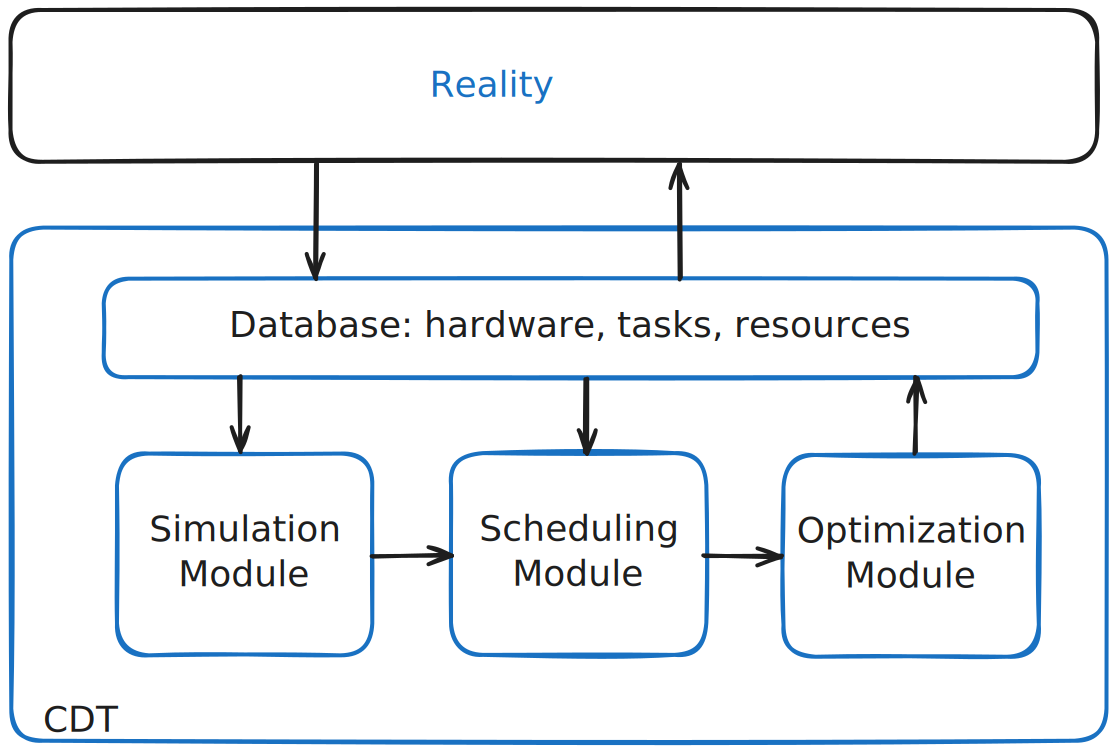
\includegraphics[width=0.8\linewidth,height=\textheight,keepaspectratio]{graphics/CDT.png}

}

\caption{\label{fig-global}Global software architecture of the CDT,
consisting of three modules: simulation (SIM), scheduling (SCD),
optimization (OPT).}

\end{figure}%

All details can be found in (Garénaux-Gruau, Bodin, and Asch 2025c).

\section*{Uncertainty}\label{uncertainty}
\addcontentsline{toc}{section}{Uncertainty}

\markright{Uncertainty}

Deterministic schedules optimize for a world that, in theory, never
materializes. Processing times vary, machines fail, networks are
overloaded, demand shifts. As a result, a schedule that is ``optimal''
under perfect information often performs poorly when reality intervenes.
Stochastic formulations, on the other hand, explicitly hedge against
variability. The resulting schedules may sacrifice some of the
theoretical efficiency, but maintain feasibility when \emph{disruptions}
occur, thus avoiding costly rescheduling or missed deadlines. Rather
than a single makespan or cost figure, one can obtain distributions:
``We meet the deadline with 95\% confidence'' which is far more
informative than ``the expected completion is Tuesday.''

Hence, when uncertainty in job durations or data transfer arrivals is
modeled, the true value of buffer capacity, parallel facilities, or
overtime flexibility becomes visible. Deterministic models
systematically undervalue these. We can compute the value of the
stochastic solution (VSS), which quantifies what can be gained by
solving the full stochastic program rather than just optimizing against
average conditions. Note that averaging yields a deterministic problem.

The Value of Stochastic Solution (VSS) is defined as the difference
between the Expectation of the Expected Value Solution (EEVS) and the
optimal objective value of the Recourse Problem (RP). The VSS quantifies
the benefit of using a stochastic model in place of a deterministic one
in decision-making problems under uncertainty. A large VSS signals that
the system is sensitive to variability, hedging decisions matter, and
the deterministic approximation is potentially dangerous.

\marginnote{\begin{footnotesize}

\[\mathrm{VSS} = \mathrm{EEV} - \mathrm{RP}\]

\end{footnotesize}}

In conclusion, when faced with expensive (financially and
environmentally), time-consuming Exascale workflows, the need to
consider uncertainty in the scheduling program is vital.
Stochastic-based scheduling can take into account any uncertain
resources and all uncertain costs---a good example would be variable
energy costs. The solution thus obtained will permit a \emph{hedging}
strategy. We can, in addition, perform risk analysis, where we compare
alternative deployments of the workflow as a function of our \emph{risk
profile}.

\bookmarksetup{startatroot}

\chapter*{Theory}\label{theory}
\addcontentsline{toc}{chapter}{Theory}

\markboth{Theory}{Theory}

\phantomsection\label{theo}

We propose a \emph{hierarchical} model for the Continuum Digital
Twin\footnote{CDT}, composed of a Supply Chain Network Design\footnote{SCND}
coupled with a Resource Constrained Process Scheduling\footnote{RCPSP}.
In such a hierarchical system, the supply chain model allocates jobs to
the best facilities, and the scheduling model then (optimally) sequences
jobs within a given facility. Supply chain optimization emphasizes
``where'' (facility location, data transfer mode, sourcing). Scheduling
emphasizes ``when'' and ``in what order.''

Recall the basic problem: given a directed graph of \(N\) storage and
processing jobs
\(\mathscr{J},\){\marginnote{\begin{footnotesize}\(\mathscr{J}=\{ J_1, J_2, \ldots J_N\},\)\end{footnotesize}}}
find an optimal allocation \(A\) and a feasible schedule \(S.\) Further
details below.

\section*{Supply Chains and
Scheduling}\label{supply-chains-and-scheduling}
\addcontentsline{toc}{section}{Supply Chains and Scheduling}

\markright{Supply Chains and Scheduling}

Let us begin by defining supply chains and scheduling in the context of
the CDT.

\begin{definition}[Supply
Chain]\protect\hypertarget{def-supp}{}\label{def-supp}

A \emph{supply chain} is a network (directed graph) of jobs, facilities,
data storage, networks, processing and end-product delivery to users.
The design poroblem is to optimally allocate an ordered list of data
storage and data processing jobs to an optimal choice of storage and
processing centres.

\end{definition}

\begin{definition}[Scheduling]\protect\hypertarget{def-sched}{}\label{def-sched}

\emph{Scheduling} is a decision-making process that deals with the
allocation of (limited) resources to tasks over given time periods. Its
goal is to optimize one or more objectives. The resulting
\emph{schedule} is a job sequence determined for every machine
(facility) of the processing system.

\end{definition}

These two models are complementary:

\begin{itemize}
\tightlist
\item
  the SCND can be used for global, over a \emph{fixed period},
  modelling---for example annualized;
\item
  the RCPSP can be used for time-dependent models, especially when
  uncertainty is introduced, as in a two-stage, or multi-stage,
  model---see below Section \textbf{?@sec-stoch}.
\end{itemize}

\begin{figure}

\centering{

\includegraphics[width=5.96in,height=1.6in]{theory_files/figure-latex/mermaid-figure-1.png}

}

\caption{\label{fig-wf}Simple directed graph (DAG) for a genomics
workflow with 4 processing jobs \(J_1,\cdots, J_4,\) and data transfers
\(c_{i,j}\) between them, including initial upload and final download.
The tasks 0 and 5 are dummy tasks, representing the start and the end of
the workflow.}

\end{figure}%

\begin{figure}

\centering{

\includegraphics[width=4.12in,height=3.29in]{theory_files/figure-latex/mermaid-figure-2.png}

}

\caption{\label{fig-wf2}Supply chain model for the CDT. For a given job,
the dataset (stored in one of two Datacentres, \(\mathrm{DC}_1\) or
\(\mathrm{DC}_2\)) can be processed on one of two HPC centres
(\(\mathrm{HPC}_1\) or \(\mathrm{HPC}_2\)), and ouput data is sent to
(and stored on) one of the two Datacentres, ready as input for the next
job. This is repeated for each job in the ordered job list (DAG).}

\end{figure}%

\section*{Supply Chain Network
Design}\label{supply-chain-network-design}
\addcontentsline{toc}{section}{Supply Chain Network Design}

\markright{Supply Chain Network Design}

\subsection*{Problem Definition}\label{problem-definition}
\addcontentsline{toc}{subsection}{Problem Definition}

Let \(\mathscr{J},\) \(\mathscr{F},\) and \(\mathscr{U}\) be respective
(finite) sets of jobs and datasets, HPC and datacentres (facilities),
and end-users. The union
\[\mathscr{N} \doteq \mathscr{J} \cup \mathscr{F} \cup \mathscr{U}\] of
these sets is viewed as the set of nodes of a directed graph
\((\mathscr{N},\mathscr{A}),\) where \(\mathscr{A}\) is a set of arcs
(directed links) connecting these nodes in a way representing flow of
the jobs---see Figure~\ref{fig-wf} and Figure~\ref{fig-wf2}. The
processing facilities \(\mathscr{F}\) can include HPC centres
\(\mathscr{H},\) data storage centres \(\mathscr{D},\) and
post-processing centres \(\mathscr{P},\)
i.e.~\(\mathscr{F}=\mathscr{H}\cup\mathscr{D}\cup\mathscr{P}.\)
Furthermore, HPC (\(i\in\mathscr{H}\)), data (\(i\in\mathscr{D}\)), and
post-processing (\(i\in\mathscr{P}\)) centers can each be composed of
sets of individual machines, \(\mathscr{M}_{i}\) and the set
\(\mathscr{F}\) includes the processing centers as well as the machines
in each center. Finally, let \(\mathscr{K}\) be the set of jobs flowing
through the ``supply chain,'\,' the digital continuum in our case.

\subsection*{State Variables}\label{state-variables}
\addcontentsline{toc}{subsection}{State Variables}

The state of the system, or supply chain, at a given time \(t,\) is
represented by state variables and coefficients:

\begin{itemize}
\tightlist
\item
  the available (open/used, or closed/unused) facilities:

  \begin{itemize}
  \tightlist
  \item
    compute centres \(x^{C}_{i}\in\left\{ 0,1\right\} ,\)
    \(i=1,\ldots,N_{C}\)
  \item
    data centres \(x^{D}_{j}\in\left\{ 0,1\right\} ,\)
    \(j=1,\ldots,N_{D}\)
  \end{itemize}
\item
  the quantity/number of jobs, or datasets, or volumes transferred

  \begin{itemize}
  \tightlist
  \item
    \(y_{ji}\) from instrument (data centre) \(j\) to compute centre
    \(i,\)
  \item
    \(y_{ij}\) from compute centre \(i\) to data centre \(j,\)
  \item
    \(y_{ik}\) from compute centre \(i\) to user \(k,\)
  \item
    \(y_{kj}\) from user \(k\) to data centre \(j,\)
  \end{itemize}
\item
  costs---both fixed and variable (eventually
  stochastic\footnote{Either a discrete set or tabulated values drawn
    from a known probability distribution, or the PDF itself.})---are
  associated with each of the decision variables;
\item
  resource supply/availability and demand/requests are specified for
  each facility, and eventually for each machine in a given
  facility---this can includes the ephemeral buffers (Garénaux-Gruau,
  Bodin, and Asch 2025a).
\end{itemize}

\subsection*{Objective Function}\label{objective-function}
\addcontentsline{toc}{subsection}{Objective Function}

The overall objective is to combine location decisions---which centres
to use---with allocation decisions---how to distribute the workloads and
jobs among the chosen centres (data and compute).

There can be a \emph{single} objective such as minimizing (any function
of) the total of fixed and variable costs, or minimizing the completion
time (makespan). \emph{Multiple} objective optimization\footnote{MOO}
seeks a tradeoff between minimum cost and maximum sustainability
(minimum environmental impact). Finally, \emph{stochastic} optimization
takes into account the uncertainties of resource availabilities and
delays, maintenance and failures, resource allocations, variable energy
costs, project costs (HR, budget).

The overall, deterministic cost function for total cost can be expressed
as a sum (some terms can be ignored by setting the coefficients to zero,
depending on the context) \begin{gather*}
\min_{x,y}\sum^{N_{C}}_{i=1}f^{C}_{i}x^{C}_{i}+\sum^{N_{D}}_{j=1}f^{D}_{j}x^{D}_{j}+\sum^{N_{C}}_{i=1}\sum^{N_{D}}_{j=1}c_{ji}y_{ji}+\\
\sum^{N_{D}}_{j=1}\sum^{N_{C}}_{i=1}c_{ij}y_{ij}+\sum^{N_{C}}_{i=1}\sum^{N_{U}}_{k=1}c_{ik}y_{ik}+\sum^{N_{U}}_{k=1}\sum^{N_{D}}_{j=1}c_{kj}y_{kj}
\end{gather*}

\begin{itemize}
\tightlist
\item
  \(f^{C}_{i},\) \(f^{D}_{j}\) are the fixed costs of using compute
  centre \(i,\) data centre \(j;\)
\item
  \(c_{ji},\) \(c_{ij},\) \(c_{ik},\) \(c_{kj}\) are the variable costs
  of the job ``flow'' from data centre \(j\) to compute centre \(i,\)
  etc. along the arc \((j,i)\in\mathscr{A}\), etc.
\item
  \(y_{ji},\) \(y_{ij},\) \(y_{ik},\) \(y_{kj}\) are the corresponding
  quantities ``flowing'' from data centre \(j\) to compute centre \(i,\)
  etc. along the arc \((j,i)\in\mathscr{A}\), etc.
\item
  \(x_{i},\) \(x_{j}\) are binary variables, indicating the choice/use
  of a particular compute or data centre;
\item
  \(N_U\) is the number of end-users;
\item
  weights, or priorities, can be attributed to each term, to either
  balance the contributions, or to give greater importance to certain
  terms.
\end{itemize}

\subsection*{Configuration Decisions}\label{configuration-decisions}
\addcontentsline{toc}{subsection}{Configuration Decisions}

We suppose that supply chain configuration decisions consist of deciding
which of the processing centers to engage, and eventually which
processing and storage machines to use within each center.

\subsection*{Mathematical Formulation - Deterministic
Model}\label{mathematical-formulation---deterministic-model}
\addcontentsline{toc}{subsection}{Mathematical Formulation -
Deterministic Model}

We begin with a deterministic formulation, and then introduce
uncertainties to obtain a full stochastic model.

Assign a binary variable \(x_{i}=1\) if the processing facility \(i\) is
engaged or machine \(i\) is used, and \(x_{i}=0\) otherwise. Operational
decisions then consist of routing the flow of all the jobs
\(k\in\mathscr{K}\) from the instrument---or primary data
reposirory---to the end-user, in a cost-optimal way, still to be
defined.

Let \(y^{k}_{ij}\) denote the flow of job \(k\) from a node \(i\) to a
node \(j\) of the network, where \((i,j)\in\mathscr{A}\) is an arc of
the network. The flow will normally be a voluminous data transfer,
possibly by even physically tansporting disk drives from remote
locations.

The optimization problem---objective function and constraints---can be
written as follows. It covers a very general case, with both optimal
allocation and eventual resource constraints.

\begin{align}
\min_{x,y} & \sum_{i\in\mathscr{F}}c_{i}x_{i}+\sum_{k\in\mathscr{K}}\sum_{(i,j)\in\mathscr{A}}q^{k}_{ij}y^{k}_{ij} \tag{1}\label{eq:sc1}\\
\textrm{s.t.} & \sum_{i\in\mathscr{N}}y^{k}_{ij}-\sum_{\ell\in\mathscr{N}}y^{k}_{j\ell}=0,\quad j\in\mathscr{F},\;k\in\mathscr{K}, \tag{2}\label{eq:sc2}\\
 & \sum_{i\in\mathscr{N}}y^{k}_{ij}\ge d^{k}_{j},\quad j\in\mathscr{U},\;k\in\mathscr{K}, \tag{3}\label{eq:sc3}\\
 & \sum_{i\in\mathscr{N}}y^{k}_{ij}\le s^{k}_{j},\quad j\in\mathscr{I},\;k\in\mathscr{K}, \tag{4}\label{eq:sc4}\\
 & \sum_{k\in\mathscr{K}}r^{k}_{j}\sum_{i\in\mathscr{N}}y^{k}_{ij}\le m_{j}x_{j},\quad j\in\mathscr{F}, \tag{5}\label{eq:sc5}\\
 & x\in\mathscr{X},\quad y\ge0, \tag{6}\label{eq:sc6}
\end{align}

\begin{itemize}
\tightlist
\item
  in \eqref{eq:sc1}, \(c_{i}\) is the cost of engaging facility \(i\) or
  using machine \(i,\) and \(q^{k}_{ij}\) is the per unit cost of
  processing job \(k\) at facility \(i\) and/or sending job \(k\) on arc
  \((i,j)\in\mathscr{A},\) (data transfer, transport and data storage
  costs)
\item
  in \eqref{eq:sc3}, \(d^{k}_{j}\) is the ``demand'' of job \(k\) at
  node \(j,\) (eg. how many CPU's or how much data storage capacity is
  required)
\item
  in \eqref{eq:sc4}, \(s^{k}_{j}\) is the ``supply'' of job \(k\) at
  node \(j,\) (eg. how many CPU's or how much data storage capacity is
  available)
\item
  in \eqref{eq:sc5}, \(r^{k}_{j}\) is the per-unit processing
  requirement for job \(k\) at node \(j,\) and \(m_{j}\) is the capacity
  of facility \(j,\)
\item
  in \eqref{eq:sc6},
  \(\mathscr{X}\subset\left\{ 0,1\right\} ^{\left|\mathscr{F}\right|},\)
  \(y\in\mathbb{R}^{\left|\mathscr{A}\right|\times\left|\mathscr{K}\right|}\)
  is a vector with components \(y^{k}_{ij},\)
\item
  all cost components are defined per given period (hour, day, week,
  month, etc.)
\end{itemize}

The above equations have the following interpretations.

\begin{itemize}
\tightlist
\item
  Objective function (\ref{eq:sc1}) minimizes the total of
  investment\footnote{CAPEX} plus operational\footnote{OPEX} costs.
\item
  \(\mathscr{K}\) represents logical dependencies and restrictions, such
  as \(x_{i}\le x_{j}\) for all \(i\in\mathscr{M}_{j},\) where
  \(j\in\left\{ \mathscr{H},\mathscr{D},\mathscr{P}\right\} ,\) which
  means that machine \(i\) should be used only if facility \(j\) is
  engaged, and since the \(x\)'s are binary the constraint
  \(x_{i}\le x_{j}\) implies that \(x_{i}=0\) if \(x_{j}=0.\)
\item
  Constraints (\ref{eq:sc2}) enforce the flow conservation of job \(k\)
  across each processing node \(j.\)
\item
  Constraints (\ref{eq:sc3}) require that the total flow of job \(k\) to
  a customer node \(j\) should exceed the ``demand'' \(d^{k}_{j}\) at
  that node.
\item
  Constraints (\ref{eq:sc4}) require that the total flow of job \(k\)
  from an instrument node \(j\) should be less than the ``supply''
  \(s^{k}_{j}\) at that node.
\item
  Constraints (\ref{eq:sc5}) enforce capacity constraints of the
  processing nodes.

  \begin{itemize}
  \tightlist
  \item
    Require that the total processing requirement of all jobs flowing
    into a processing node \(j\) should be smaller than the capacity
    \(m_{j}\) of facility\(j\) if it is used (\(x_{j}=1\)).
  \item
    If facility \(j\) is not used (\(x_{j}=0\)), the constraint will
    force all flow variables \(y^{k}_{ij}=0\) for all
    \(i\in\mathscr{N}.\)
  \end{itemize}
\item
  Finally, constraint (\ref{eq:sc6}) enforces the feasibility constraint
  \(x\in\mathscr{X}\) and the non-negativity of the flow variables
  corresponding to an arc \((i,j)\in\mathscr{A},\) and job
  \(k\in\mathscr{K}.\)
\end{itemize}

We can rewrite the above in a very compact, matrix-vector form.

\begin{align*}
\min & \,\,c^{\top}x+q^{\top}y\\
\textrm{s.t.} & \,\,Ny=0,\\
 & Cy\ge d,\\
 & Sy\le s,\\
 & Ry\le Mx,
\end{align*} where

\begin{itemize}
\tightlist
\item
  vectors \(c,\) \(q,\) \(d,\) and \(s\) represent fixed costs,
  processing or transmission costs, demands, supplies, respectively;
\item
  matrices \(N,\) \(C,\) and \(S\) correspond to summations of the
  respective expressions, (nodes, demands, supplies);
\item
  \(R\) is the matrix of \(r^{k}_{j}\) (requirements);
\item
  \(M=\textrm{ diag }(m_{j})\) (machine capacities).
\end{itemize}

\subsection*{Simplified Cases}\label{simplified-cases}
\addcontentsline{toc}{subsection}{Simplified Cases}

The above formulation covers both the cost-optimal streaming of jobs
across the cyberinfrastructure as well as the respect of individual
facilities' constraints. The latter is a resource-constrained scheduling
problem.

\textbf{Unconstrained-Resource Problem}

As a first simplification, we suppose that the facilites possess the
necessary capacities to service the requirements of all the incoming
data storage and processing jobs. Suppose that we still have fixed and
variable costs, so the objective does not change. The
``infinite-resource'' problem simplifies to:

\begin{align}
\min_{x,y} & \sum_{i\in\mathscr{F}}c_{i}x_{i}+\sum_{k\in\mathscr{K}}\sum_{(i,j)\in\mathscr{A}}q^{k}_{ij}y^{k}_{ij} \tag{1a}\label{eq:sc1a}\\
\textrm{s.t.} & \sum_{i\in\mathscr{N}}y^{k}_{ij}-\sum_{\ell\in\mathscr{N}}y^{k}_{j\ell}=0,\quad j\in\mathscr{F},\;k\in\mathscr{K}, \tag{2a}\label{eq:sc2a}\\        
 & x\in\mathscr{X},\quad y\ge0, \tag{6a}\label{eq:sc6a}
\end{align}

\textbf{Resource-Constrained Project Scheduling Problem (RCPSP)}

A second simplification is to consider the resource constraint problem,
without facility or machine allocations. The Resource-Constrained
Project Scheduling Problem (RCPSP) is a combinatorial optimization
problem that consists of finding a feasible scheduling for a set
of~\(n\)~jobs subject to resource and precedence constraints. Each job
has a processing time, a set of successor jobs and a required amount of
different resources. Resources may be scarce but are renewable at each
time period. Precedence constraints between jobs mean that no jobs may
start before all its predecessors are completed. The jobs must be
scheduled non-preemptively, i.e., once started, their processing cannot
be interrupted.

The RCPSP has the following input data:

\begin{itemize}
\tightlist
\item
  \(\mathcal{J}\) set of jobs.
\item
  \(\mathcal{R}\) set of renewable resources.
\item
  \(\mathcal{S}\) set of precedences between
  jobs~\((i,j)\in\mathcal{J}\times\mathcal{J}.\)
\item
  \(\mathcal{T}\) planning horizon: set of possible processing times for
  jobs.
\item
  \(p_{j}\) processing time of job~\(j.\)
\item
  \(u_{(j,r)}\) amount of resource~\(r\)~required for processing
  job~\(j.\)
\item
  \(c_{r}\) capacity of renewable resource~\(r.\)
\end{itemize}

A binary programming formulation was proposed by Pritsker et al.~in
1986. In this formulation, decision variables \(x_{jt}=1\) if job \(j\)
is assigned to begin at time \(t\); otherwise, \(x_{jt}=0.\) All jobs
must finish in a single period of time without violating precedence
constraints while respecting the amount of available resources. The
model proposed by Pristker can be stated as follows:

\begin{alignedat}{1}\textrm{Minimize} & \sum_{t\in\mathcal{T}}t\cdot x_{(n+1,t)}\\
\textrm{Subject to:} & \sum_{t\in\mathcal{T}}x_{(j,t)}=1\,\,\,\forall j\in J,\\
 & \sum_{j\in J}\sum^{t}_{t_{2}=t-p_{j}+1}u_{(j,r)}x_{(j,t_{2})}\leq c_{r}\,\,\,\forall t\in\mathcal{T},r\in R,\\
 & \sum_{t\in\mathcal{T}}t\cdot x_{(s,t)}-\sum_{t\in\mathcal{T}}t\cdot x_{(j,t)}\geq p_{j}\,\,\,\forall(j,s)\in S,\\
 & x_{(j,t)}\in\{0,1\}\,\,\,\forall j\in J,t\in\mathcal{T}.
\end{alignedat}

\textbf{Mutli-Project Multi-Mode RCPSP}

Note that the above formulation is restricted to temporal scheduling on
a \emph{single} machine, and for a single project, or collection of
jobs. This formulation has been generalized to deal with multiple
machines and multiple projects. In this case, the formulation becomes
very similar to that of a supply chain. It is referred to in the
literature as the \emph{multi-mode resource-constrained multi-project
scheduling problem}, or MRCMPSP. We can then perform simultaneous
scheduling of a set of multiple projects taking into account the
availability of local and global resources under different time and
resource constraints. This has practical importance, at national and
European levels, when cross-facility implies exploitation of
cyberinfrastructure resources across different countries, for example,
as would be the case for EuroHPC\footnote{
  \url{https://www.eurohpc-ju.europa.eu/}}, at the European level, or
GENCI\footnote{ \href{https://www.genci.fr/}{https://www.genci.fr//}}
for France. Imagine being able to plan and pilot multiple exascale
projects, on multiple sites, over multiple countries\ldots{}\footnote{These
  would be multiple states, in the USA context.}

This general formulation is then mathematically equivalent to the supply
chain configuration problem\footnote{SCCP} with resource constraints.
The loop is closed.

\section*{Optimization}\label{optimization}
\addcontentsline{toc}{section}{Optimization}

\markright{Optimization}

In summary, this book has no content whatsoever. In summary, this book
has no content whatsoever.

\subsection*{MILP formulations for RCPSP and
SCND}\label{milp-formulations-for-rcpsp-and-scnd}
\addcontentsline{toc}{subsection}{MILP formulations for RCPSP and SCND}

We consider single- and multi-mode resource-constrained project
scheduling problems. In summary, this book has no content whatsoever.

\subsection*{Precedence Constraints}\label{precedence-constraints}
\addcontentsline{toc}{subsection}{Precedence Constraints}

In summary, this book has no content whatsoever. In summary, this book
has no content whatsoever.

\subsection*{Disjunctions}\label{disjunctions}
\addcontentsline{toc}{subsection}{Disjunctions}

In summary, this book has no content whatsoever. In summary, this book
has no content whatsoever.

\section*{Uncertainty}\label{sec-stoch}
\addcontentsline{toc}{section}{Uncertainty}

\markright{Uncertainty}

In practice some of the scheduling parameters may be uncertain. The
exact duration of an activity, for instance, might not be known at the
beginning of the project. Similarly, the number of available resources
is another parameter that may not be known before project execution.
These uncertainties may be due to different sources, including
estimation errors, unforeseen (weather) conditions, late ``delivery''
(unavailability) of some required resources, unpredictable incidents
such as machine breakdown or worker accidents, etc.

\bookmarksetup{startatroot}

\chapter*{Examples}\label{examples}
\addcontentsline{toc}{chapter}{Examples}

\markboth{Examples}{Examples}

\phantomsection\label{exam}

In summary, this book has no content whatsoever.

\section*{Examples}\label{examples-1}
\addcontentsline{toc}{section}{Examples}

\markright{Examples}

In summary, this book has no content whatsoever.

\begin{figure}

\centering{

\pandocbounded{\includegraphics[keepaspectratio]{examples_files/figure-latex/fig-line-plot-output-1.pdf}}

}

\caption{\label{fig-line-plot}A line plot}

\end{figure}%

We observe in Figure~\ref{fig-line-plot} that there is a clear trend, up
and down.

\section*{Use-Cases}\label{use-cases}
\addcontentsline{toc}{section}{Use-Cases}

\markright{Use-Cases}

\subsection*{Setup and Linear Programming
Example}\label{setup-and-linear-programming-example}
\addcontentsline{toc}{subsection}{Setup and Linear Programming Example}

As an introduction we load the necessary \texttt{pyomo} packages and
solve an ultra-simple linear programming example. \[
\begin{array}{ll}
  \min       & 2 x_1 + 3 x_2\\
  \mathrm{s.t.} & 3 x_1 + 4 x_2 \geq 1\\
             & x_1, x_2 \geq 0
\end{array}
\]

\begin{itemize}
\tightlist
\item
  \texttt{pyomo.environ} provides the framework for building the model
\item
  \texttt{SolverFactory} allows to call the solver used to solve the
  optimization problem
\end{itemize}

\begin{verbatim}
x = (0.33, 0.00)
optimal value = 0.67
\end{verbatim}

We can print out

\begin{itemize}
\tightlist
\item
  the complete model;
\item
  a full trace of the optimization process.
\end{itemize}

(use collapsed display here - click to expand and view output)

\subsection*{Precedence Example}\label{precedence-example}
\addcontentsline{toc}{subsection}{Precedence Example}

We illustrate how to set up a \emph{precedence table}, made up of job
pairs that define pairwise precedences.

\subsection*{Disjunctions}\label{disjunctions-1}
\addcontentsline{toc}{subsection}{Disjunctions}

When faced with a choice among exclusive options, we resort to
disjunctive programming, based on:

\begin{itemize}
\tightlist
\item
  Big-M formulation.
\item
  Logical formulation.
\end{itemize}

\subsection*{Simplified Supply Chain
Example}\label{simplified-supply-chain-example}
\addcontentsline{toc}{subsection}{Simplified Supply Chain Example}

Putting together:

\begin{itemize}
\tightlist
\item
  precedence
\item
  TBC
\end{itemize}

\subsection*{Simplified RCPSP Example}\label{simplified-rcpsp-example}
\addcontentsline{toc}{subsection}{Simplified RCPSP Example}

Putting together:

\begin{itemize}
\tightlist
\item
  precedence
\item
  TBC
\end{itemize}


\backmatter


\end{document}
